% ------------------------------------------------------------------------
% ------------------------------------------------------------------------
% ------------------------------------------------------------------------
%\chapter{MCQMC 2012}



\chapter{Practical Information}



\section{Conference Venue}
MCM 2025 is hosted by Illinois Institute of Technology (Illinois Tech).  All talks will take place on the Mies Campus in the following three buildings
\begin{itemize}
	\item Hermann Hall (HH),
	\item Perlstein Hall (PH), and
	\item Wishnick Hall(WH)
\end{itemize}
See the campus map on the next page or at \href{https://www.iit.edu/sites/default/files/2022-08/mies-campus-accessibility-map-2022.pdf}{this link}.  


\section{Getting to Illinois Tech}
Illinois Tech is located several miles south of downtown  can reach Illinois Tech via 
\begin{itemize}
	\item the Chicago Transit Authority (\href{https://www.transitchicago.com/schedules/}{CTA}) `L' Green or Red Lines, which stop at 35th Street, 
	\item the href{https://www.transitchicago.com/schedules/}{CTA} Route 29 bus, which stops at the corner of State and 32nd Streets, or
	\item taxi, Uber, or Lyft.
\end{itemize}

Two major airports, \href{https://www.flychicago.com/ohare/home/Pages/default.aspx}{O'Hare} and \href{https://www.flychicago.com/midway/pages/default.aspx}{Midway} serve Chicago, and are not far from Illinois Tech.

\clearpage

\begin{center}
	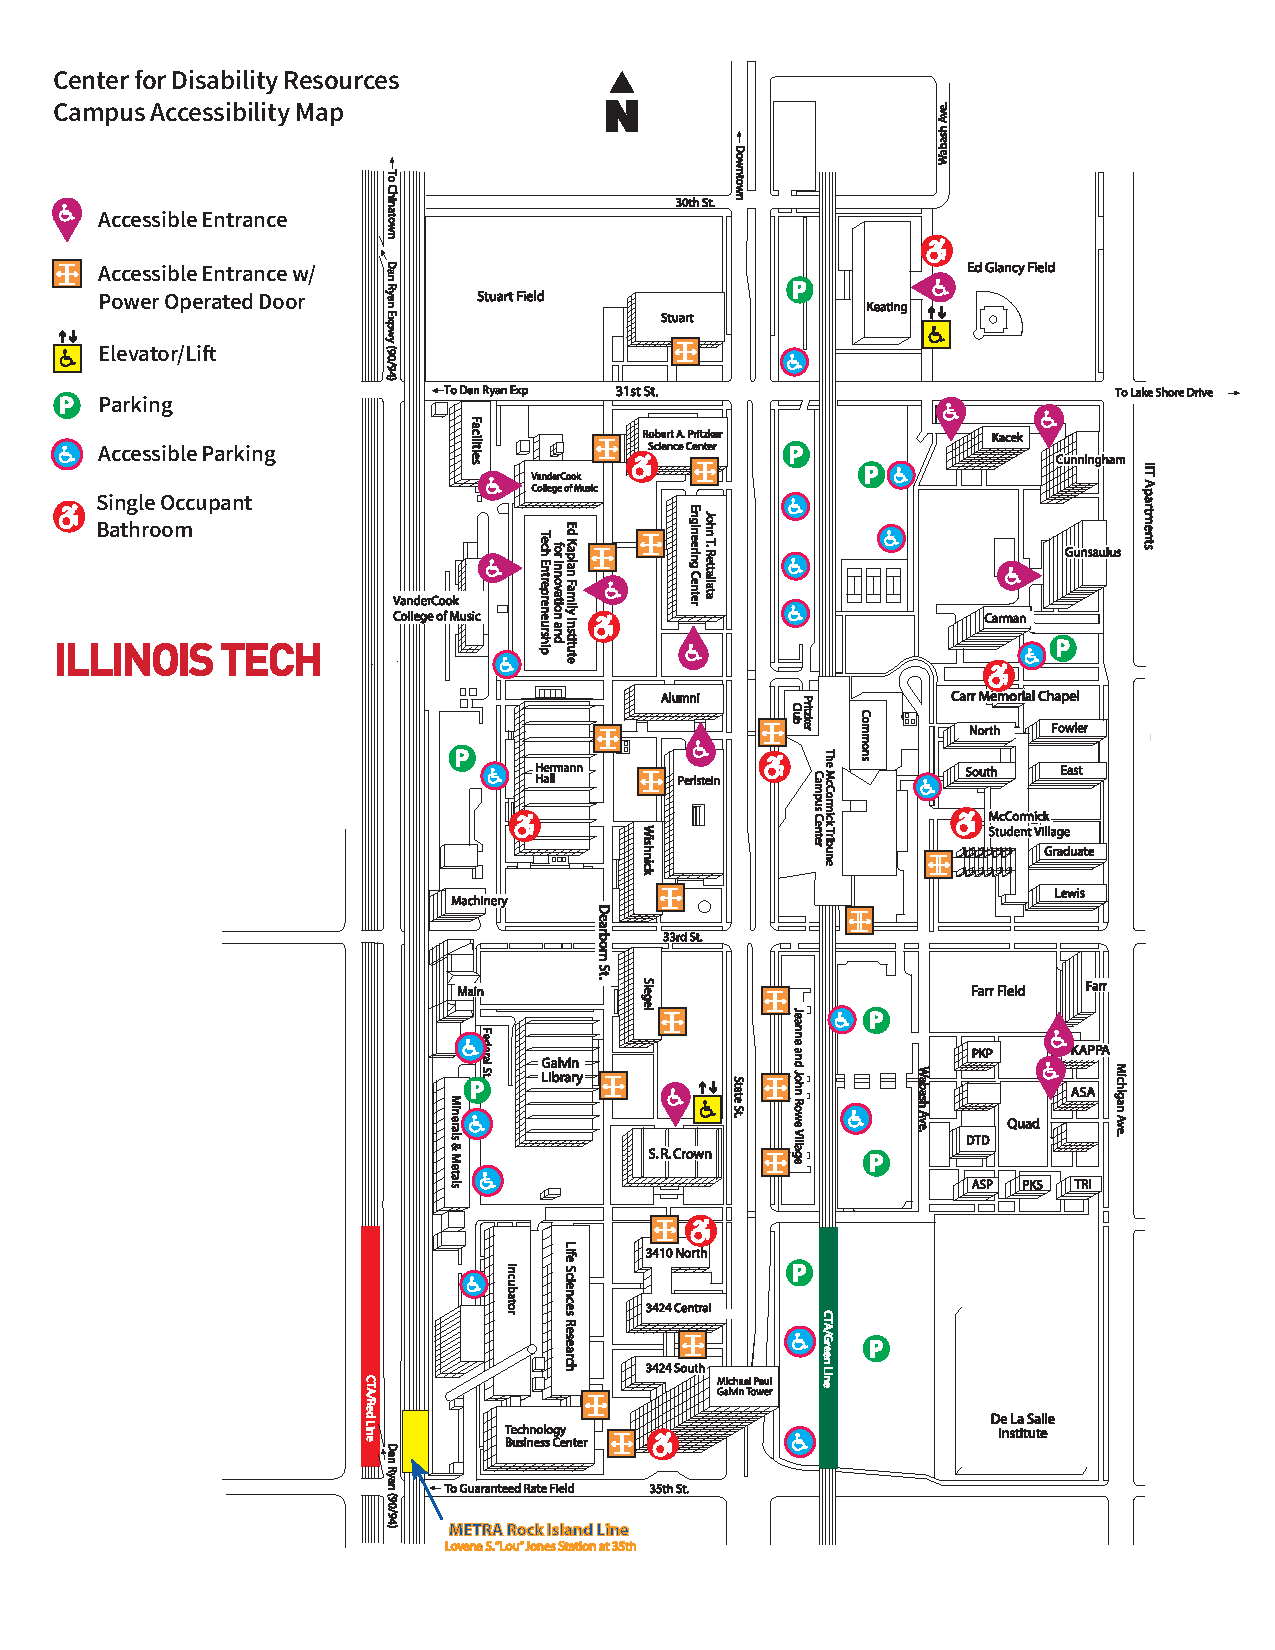
\includegraphics[width = \textwidth] {Photos/mies-campus-accessibility-map-2022.pdf}
\end{center}




\subsubsection{Conference Schedule}

The conference schedule included in this program book may not reflect last-minute changes to the schedule. The online version of the schedule on the conference website
will be kept as much up-to-date as possible, reflecting also last minute changes. 

\subsubsection{Registration and Information Desk}

The registration and information desk is located in the STC 1st floor foyer, outside of STC 1012.
Sunday afternoon registration will take place from 13:30 to 16:00 on August 18. Monday (August 19) morning registration will take place from
08:00 to 12:30 and from 14:00 to 16:00 on. There will be support on site throughout the week for participants who arrive after Monday. 


\subsubsection{Sunday Tutorials}

Sunday afternoon tutorials will be held in STC 1012, and are given by 
Fred Hickernell (14:15--15:45) and Peter Frazier (16:00--17:30). 


\subsubsection{Opening Ceremony}

The opening ceremony will be held in STC 1012 on Monday, August 19,
at 08:45, before the first plenary talk.

\subsubsection{Plenary Talks}

Plenary talks will be held in STC 1012. Plenary talks are 50 minutes long, plus 10 minutes for questions and discussions. Due to the
tight conference schedule, we kindly ask the chairs to strictly
observe the time constraints.

\subsubsection{All other talks}

All other talks (except plenary talks and tutorials) will be held in 
parallel sessions in STC 0020, STC 0040, STC 0050, and STC 0060. These talks 
are 25 minutes long plus 5 minutes
for questions and discussions. Due to the tight
conference schedule, we kindly ask all speakers and chairs to strictly observe
the time constraints.


\subsubsection{Coffee Breaks}

Morning and afternoon coffee breaks will take place in the STC lower-level atrium, between the plenary talk and parallel sessions, i.e., from 10:00 to 10:30 and from 15:00 to 15:30. There will also be a coffee break on Sunday August 18 between the two tutorials, from 15:45 to 16:00.


\subsubsection{Reception (Monday)}

On Monday, August 19, there will be a welcome reception from 18:00 to 19:30.
Drinks and finger food will be provided in the Mathematics 3 (M3) building atrium (ground floor). 
M3 is just north of the Mathematics \& Computing (MC) building. 
%Heading on Ring Road from STC, turn right and go on the path immediately after the Quantum Nano Centre (QNC), and then continue around MC until M3.
Please refer to the conference website for campus maps or see above information on Location.


\subsubsection{Award Ceremony of the Journal of Complexity (Monday)}

On Monday, August 19, there will be a short ceremony to award IBC Awards and IBC Young Researcher Awards of the Journal of Complexity. 
The ceremony will be chaired by senior editors of the journal, and take place at about 8:55 in STC 1012
(immediately before the first plenary talk).


%\subsubsection{Editorial Board Meeting of the Journal of Complexity (Tuesday)}

%On Tuesday, August 20, the members of the Editorial Board of the Journal of Complexity will have a closed meeting at 19:00. 
%If you have any comments or suggestions regarding the journal, please approach any member of the Editorial Board
%prior to this meeting. The meeting will take place at .....

\subsubsection{Conference Photo (Wednesday)}

A conference photo will be taken on Wednesday, August 21, at 17:30, right after the afternoon parallel sessions. Details will be announced 
during the conference week.



\subsubsection{Conference Dinner (Wednesday)}

The conference dinner will take place in the Engineering 7 (E7) building, which is outside of Ring Road, immediately behind and directly connected from inside to the Engineering 5 (E5) building. You can find it easily as E5 is the building connected to campus by a bridge going over Ring Road near the Davis Centre. 

Please note that all participants (conference participants and accompanying persons) must be registered in advance for this event.


\subsubsection{Steering Committee Meeting (Thursday)}

On Thursday, August 22, the MCQMC Steering Committee will have a closed meeting, starting at 19:00. If
you have any comments or suggestions, or would like to propose hosting a
future conference, please approach any member of the Steering Committee
prior to this meeting. 



%--------------------------------

\iffalse
\subsection{Covid-19 Rules}

The Covid-19 situation has relaxed considerably over the past months in most of Europe, but there are a few Covid rules that 
we kindly ask you to observe.
\begin{itemize}
 \item Even though there is no strict mask mandate on JKU campus any longer, there is a strong recommendation to wear masks in crowded places. We 
 fully support this recommendation and ask you to \textbf{wear masks} whenever you are within larger groups of people. 
 \textbf{Every conference participant will find an FFP2 mask in their conference kit. Please use it.}
 \item Should you suspect that you might have contracted Covid-19, please \textbf{do not} come to the conference 
 venue \textbf{under any circumstances}, but make yourself known to the conference organizers. Call the Austrian Agency for Health at +43-732-1450, where you 
 will be assisted with organizing a PCR test and all further steps.
 \item If you should show symptoms typical of Covid-19 but are not sure 
 whether you might have Covid or a cold or flu, \textbf{do not} come to the conference until you have a negative PCR test result. 
 \item In any case, please use common sense, and try to help us in keeping MCQMC 2022 Covid-19 free. 

 
\end{itemize}
\fi


%--------------------------------

\subsubsection{Food}

Lunch will \emph{not} be provided. There will be a Tim Horton's (located in the Davis Centre (DC) ground floor), Subway and Flock Stop (both located in the Student Life Center - SLC ground floor), open on-campus during the week providing an inexpensive option for lunch.  
Alternatively, a short 10-minute walk east from STC leads to the ``University Shops Plaza" where there are several restaurants and fast-food outlets providing more diverse options for conference participants. Another popular lunch venue is Ken Sushi House on Phillip Street, just east of campus.

\iffalse
\arrayrulecolor{black}

\begin{center}
\begin{footnotesize}
 \begin{longtable}{|| l || l | l | l l||} 
 \hline
 \hline  
  1A & \textbf{JKU Mensa}  & \url{www.mensen.at}  & Mon--Fri & 11:00--13:30  \\ \hline
  1B & \textbf{Cafe Ch@t} & Keplergeb\"{a}ude &  Mon--Thu & 08:00--19:00 \\
     &                    &                         &  Fri & 08:00--14:00 \\ \hline
  1C & \textbf{Science Cafe} & Science Park 3 &  Mon--Thu & 08:00--16:00 \\ 
     &                    &                         &  Fri & 08:00--14:00 \\ \hline
  1D & \textbf{Cafe Sassi} & Bankengeb\"{a}ude &  Mon--Thu & 08:00--16:00 \\
     &                    &  \url{www.sassi.at}  &  Fri & 08:00--14:00 \\ \hline
  1E & \textbf{Teichwerk} & University pond &  Mon--Thu & 08:00--16:00 \\
     &                    & \url{www.dasteichwerk.at}  &  Fri & 08:00--14:00 \\ \hline
  2  & \textbf{KHG Mensa} & Mengerstr. 23 & Mon--Fri & 11:00--13:00  \\ 
  
     &                    & \texttt{https://www.dioezese-linz.at/} & & \\
     &                    &  \texttt{khg/mensa/menueplan}  & & \\ \hline
  3  & \textbf{Winklermarkt} &  Altenbergerstr. 40 & Mon--Thu & 07:30--18:30 \\
     & (Supermarket \& &  \texttt{https://winklermarkt.at/}  & Fri & 07:30--19:00 \\
     & Restaurant) &  \texttt{menuplan/}  & Sat & 07:30--17:00 \\ \hline
  4a  & \textbf{Pizzeria} & Aubrunnerweg 1a & Mon--Sun & 11:00--15:00 \\
     & \textbf{Bella Casa} & Phone: +43-732-245646 &          & 17:00--24:00 \\ \hline
  4b  & \textbf{Chinese Restaurant} & Aubrunnerweg 11 & Mon--Sun & 11:00--14:30 \\
     & \textbf{Jadegarten} & Phone: +43-732-750160 &          & 17:00--23:00 \\ \hline
  5  & \textbf{Restaurant} & Altenbergerstr. 6--8 & Mon--Thu & 10:30--22:00 \\
     & \textbf{Burgerista} &  Phone: +43-50-666666 &  Fri--Sat & 10:30--23:00 \\ 
     &  &                     &  Sun & 10:30--23:00 \\ \hline
  6  & \textbf{Restaurant} & Freist\"{a}dter Str. 297 & Mon--Sat & 11:00--23:00 \\
     & \textbf{Peter's Platz} &  Phone: +43-732-251112                   &  Sun & 11:00--17:00 \\ \hline
  7 & \textbf{Subway} & Freist\"{a}dter Str. 313 & Mon--Sun & 11:00--22:00 \\ \hline
  8  & \textbf{Asian Restaurant} & Freist\"{a}dter Str. 315 & Tue & 11:30--14:30 \\
     & \textbf{Ost18} &  Phone: +43-732-244042              &  Wed--Mon & 11:30--14:30 \\ 
     &  &   &   & 17:30--23:00 \\ \hline
  9  & \textbf{Raab Mensa} & Julius-Raab-Str. 10 & Bar: & \\
     & (Restaurant \& Bar)   & Phone: +43-732-24570 & Mon--Thu & 06:30--23:30\\
     &             & \texttt{www.sommerhaus-hotel.at/} & Sat--Sun & 06:30--11:00 \\
     &                            & \texttt{de/linz\#{}speiseplan} & Restaurant:& \\
     &                            &  & Mon--Sun & 11:30--14:30\\
     &                            &  &  & 17:00--21:00\\ \hline
 10  & \textbf{McDonald's \&} & Freist\"{a}dter Str. 298 & Sun--Thu & 07:00--00:00 \\
     & \textbf{McCafe} &               &  Fri--Sat & 07:00--02:00 \\ \hline
 11  & \textbf{``Penny''} & J.W.-Klein-Str. 58 & Mon--Fri & 07:40--20:00 \\
     & (Supermarket)      &                    & Sat      & 07:40--18:00 \\ \hline 
 12  & \textbf{``Hofer''} & Freist\"{a}dter Str. 401 & Mon--Fri & 07:40--20:00 \\
     & (Supermarket)      &                    & Sat      & 07:40--18:00 \\ \hline 
 13  & \textbf{``Billa''} & Freist\"{a}dter Str. 400 & Mon--Fri & 07:40--20:00 \\
     & (Supermarket)      &                    & Sat      & 07:40--18:00 \\ \hline      
 14  & \textbf{``Spar''} & Altenbergerstr. 69 & Mon--Fri & 07:30--19:45 \\
     & (Supermarket)      &  (on JKU campus)  & Sat      & 08:00--18:00 \\ \hline  
\hline   
\end{longtable}
\end{footnotesize}
\end{center}
\fi


%\begin{center}
% \includegraphics[width=14cm]{Food_map}
%\end{center}



\subsubsection{Travel to Waterloo from Toronto Pearson Airport (YYZ)}

Before you travel to Canada, please ensure you have the proper documents and visitor visas to visit. Check the \href{https://www.canada.ca/en/immigration-refugees-citizenship/services/visit-canada.html?outside}{Government of Canada website} for specific requirements for your country.

Details regarding travel visas can be found on the \href{https://uwaterloo.ca/monte-carlo-methods-scientific-computing-conference/registration}{registration page}.

Waterloo is located approximately one hour by car from Toronto Pearson Airport, however there are several methods to book travel from the airport to Waterloo.

\begin{itemize}
\item By Bus: There are buses that travel between Toronto Pearson YYZ, to Waterloo. \href{https://www.gotransit.com/en}{GO Transit} is the most popular.
\item By Taxi: With Waterloo Taxi, you can reserve a taxi on the \href{https://waterlootaxi.ca/mobile/airport.php}{Waterloo Taxi online form} or call at +1 (519) 888-7777.
\item By Rail: UP Express is a direct journey from Toronto Pearson International Airport to Union Station, Downtown Toronto. When at Union Station, transfer to \href{https://www.viarail.ca/en}{VIA Rail} train or \href{https://www.gotransit.com/en}{GO train}.
\item By Airways Transit (up to 8 passengers): Reserve door-to-door service on the \href{https://www.airwaystransit.com/Private-Service/}{Airways Transit} website.
By Car: Take ON-401 W towards London and then take exit 278 to merge onto ON-8 W toward Kitchener/Waterloo.
\end{itemize}



\subsubsection{Public transport in Waterloo}

By Bus: \href{https://www.grt.ca/en/index.aspx}{Grand River Transit} is the public transit operator for the Region of Waterloo, Ontario. It operates daily bus serves across Waterloo and the University of Waterloo campus.

By \href{https://www.grt.ca/en/ion-light-rail.aspx}{ION Light Rail} Travel: ION is Waterloo Region’s light rail transit (LRT) system. It runs between Kitchener’s Fairview Park Mall and Waterloo’s Conestoga Mall, with stops at the University of Waterloo campus. ION trains connect passengers to the existing bus system (Grand River Transit), making it easy to travel across the region.



\subsubsection{Equipment in classrooms used for conference}

Each lecture hall is equipped with a desktop computer running Windows,
with USB port access and internet connection, a data projector and screen, 
and blackboards. One MCQMC staff member 
%(with a yellow name tag) 
will be present 
in each lecture hall to assist with IT related issues.

We strongly encourage you to make yourself known to your session chair and (if necessary) 
the MCQMC staff member assigned to your lecture room, prior to your talk. Please prepare your talk in the form of a PDF or PPT document. A slides repository will be created shortly before the conference to facilitate the uploading of slides to the desktop computer in each room prior to each session by MCQMC staff. More detailed instructions will be sent to speakers and session chairs prior to the conference. An alternative option is to bring 
a USB storage device with your slides copied on it and make sure that your talk is copied onto
the desktop computer during the break prior to your talk. 
%We cannot guarantee 
%that other file formats than PDF can be displayed correctly.

If you require access to other software packages or other audio-visual
equipment, please communicate with the conference organizers well ahead of time to
see if it can be arranged. It is possible to connect your personal laptop
to the data projector, but we prefer that you avoid this option due to the
tight conference schedule. If you need to use your own laptop, please make
sure that you discuss this with a MCQMC staff member %assigned to your room 
and 
that you test the connection well before your talk.


\subsubsection{Internet and Computer Access}

University of Waterloo has eduroam to provide free wireless access for visitors whose home
institutions also have eduroam. For more information on eduroam see
\url{http://www.eduroam.org}. Please check with your institution whether you have access to eduroam and
for instructions on how to set up eduroam (this depends on your home
institution and not on local institutions).

If you cannot use eduroam, conference participants will be granted access to the Waterloo wireless network on campus via self-registration. Further details on how to do so will be announced during the opening of the conference. 

%Please note that we are unable to set up new accounts at the conference.

In any case, please use the wireless connections provided responsibly. 



%\subsection{Printing and Photocopying}

%The main library of JKU offers the possibility to print, copy, and scan for guests; you will have to pay a fee. All further information can be obtained from the main desk of the JKU library.

%Alternatively, conference organizers may be willing to help you with a small amount of printing or photocopying. We ask for your understanding, though, that we cannot provide this as a regular service, but only in exceptional cases. 




\subsubsection{Emergency Contacts, Hospitals and Services on Campus}

The emergency phone number in Canada is \textbf{911}. For emergency calls on-campus, call the UW Special Constable at 519-888-4911. There is a Special Constable on campus 24 hours a day, 7 days a week.


\textbf{Local Kitchener-Waterloo Hospitals}

\begin{itemize}
    \item Grand River Hospital, 835 King Street West, Kitchener (519-742-3611)

    \item St. Mary’s General Hospital, 911 Queen’s Boulevard, Kitchener (519-744-3311)
\end{itemize}




\subsubsection{Power Plugs in Canada}

In Canada, the standard power sockets are:

\begin{itemize}
    \item Type A:
    \begin{itemize}
        \item Description: This socket has two flat parallel pins.
        \item Voltage: 120 V
        \item Frequency: 60 Hz
    \end{itemize}

    \item Type B:
    \begin{itemize}
        \item Description: This socket has two flat parallel pins and a grounding pin (three-pronged).
        \item Voltage: 120 V
        \item Frequency: 60 Hz
    \end{itemize}
\end{itemize}

%\begin{center}
%\includegraphics[width=5cm]{Power_Pic}
%\end{center}

\subsubsection{Closing of the Conference}

MCQMC 2024 will be closed with a few short announcements and remarks
immediately after the final parallel sessions, which finish at 12:30 on Friday, August 23.
%.... There will also be a short presentation about MCQMC 2026 (?)



\subsubsection{Proceedings}

Following the tradition of the MCQMC conference series, a selection of
strictly refereed papers will be published after the conference as a
Springer book. Every speaker is welcome to submit a paper based on
his/her talk, with the length strictly not exceeding 16 pages in the Springer style. 
Plenary and tutorial speakers are invited to submit papers of at most 30 pages length. The papers of 
plenary and tutorial speakers can be survey articles.

The submission deadline for manuscripts is December 13, 2024. Please send your submissions as a pdf file 
to \texttt{mcqmc.2024@uwaterloo.ca}.

Further instructions will be provided in the closing session of the conference, and will be available on the conference
website later.

\subsubsection{Conference Statistics (as of July 5)}

\begin{center}
 \begin{tabular}{ll}
 Number of participants & 151 \\
 Number of plenary lectures & 8 \\
 Number of tutorials & 2 \\
 Number of talks & 137 \\
 Number of special sessions & 24 (85 talks) \\
 Number of technical sessions & 12 (42 talks) \\
 \end{tabular}
\end{center}